\documentclass[a4paper,10pt,oneside]{book}

% packages 
\usepackage{arsclassica}    % fancy layout
\usepackage[english]{babel}\addto{\captionsenglish}{\renewcommand{\bibname}{References}}
\usepackage{caption}         % figure captions
\usepackage[square,numbers,super,sort&compress]{natbib}  % bibliography style
\usepackage[cc]{titlepic}    % enable logo on title page
\usepackage{graphicx}       % logo related

\usepackage{standalone}
\standalonetrue

% Margins for pretty version ::
%\usepackage[pass]{geometry}
% Margins for university regulations ::
\usepackage[top=2cm, bottom=4cm, left=4cm, right=2.5cm]{geometry}
\usepackage{setspace}
\onehalfspacing

% don't hang captions
\captionsetup{format=plain}

% bibliography
\bibliographystyle{../thesis}

% title setup
\title{ \vspace{3in} Unravelling higher order genome organisation {\small [working
    title]} \\ \vspace{2em} {\large {\bf Introduction}} }
\author{Benjamin L. Moore}
\titlepic{\vspace{2.2in} 
\includegraphics[width=\textwidth]{/Users/benmoore/hvl/1yrReport/figs/igmm.png}}

\begin{document}

%\maketitle

\chapter{Introduction}
\section{Genome organisation}
%
%It's oft-stated that the DNA within each human cell would extend for two metres fully extended. Instead that same length of DNA packs into a cell nucleus with a diameter in the order of micrometers ($\mu$m). This is achieved through a complex organisation hierarchy, ranging from how chromosomes are arranged in the nucleus, down to how DNA is wrapped around nucleosomes.\cite{Pombo2015}
%
%Briefly, DNA exists mostly as a left-handed double-helix of hydrogen bonded purines and pyrimidines. These in turn are wrapped around histone octamers, proteins with tuneable DNA packing properties. These wrapped histones can be visualised as "beads on a string" in transcriptionally active regions, and possibly as a more-compact 30 nanometre fibre, though this is disputed.\cite{Naumova2013} %citations therein

\subsection{C-methods and Hi-C}

Classical studies of chromosome conformation relied on microscopy techniques to visualise nuclear architecture, most commonly fluorescence \emph{in situ} hybridisation (FISH). These techniques led to the discovery of ``chromosome territories", regions of the nucleus wherein distinct chromosomes were thought to occupy, and more broadly identified the non-random arrangement of loci in three-dimensional space.\cite{DeWit2012, VanSteensel2010} Finer details of chromatin organisation, such as the proposed 30 nm fibre, were also introduced through microscopy-based techniques. Techniques such as FISH are powerful for precise inspection of single genes, but are low-throughput and offer limited resolution.\cite{DeWit2012}

With the advent DNA sequencing technology, new experimental methods emerged. Chromosome conformation capture (3C), introduced by Dekker \emph{et al.}\cite{Dekker2002} was the first sequencing-based method of measuring chromosome conformation. The method uses formaldehyde to cross-link nuclear proteins in place, trapping genomic regions that were physically co-located through bound proteins, then to apply a frequent restriction enzyme to shear the sample into fragments. Next, under dilute conditions, DNA fragments are ligated together. The dilute conditions favour ligations between fixed fragments, with the aim of generating hybrid fragments form two genomic regions which were close together in the original preparation. Cross-linking can then be reversed and, in the case of the original 3C method, measured by quantitative PCR using pre-designed primers for your fragments of interest. The end result is a relative measure of interaction frequency between any two regions of interest, in theory directly proportional to their distance in three-dimensional space.

The rapid advancement of sequencing, allowed the original 3C method to be further developed, first through microarray technology, then using high-throughput sequencing. Two protocols were proposed for a 3C-inspired one-to-many assay\cite{Zhao2006, Simonis2006} (both named 4C), whereby interactions were measured for a specific ``viewpoint" fragment against all other restriction fragments genome-wide. The same year a many-to-many assay (5C) allowed measurements for all restriction fragments within a specified region.\cite{Dostie2006} 

The final step was an all-versus-all assay, capable of assaying pairwise interaction frequencies between all restriction fragments of a genome. This assay was published by Lieberman Aiden \emph{et al.}\cite{Lieberman2009} and named Hi-C (Fig. \ref{fig:hicmethod}). The Hi-C method added biotin tagging to pull-down only ligated fragments for sequencing. At the time of publication, resolution of Hi-C data for analysis was limited by sequencing depth, given the huge number of restriction fragments produced by a 6-cutter enzyme (HindIII and NcoI were used in \cite{Lieberman2009}) but the falling costs of sequencing and proven utility of the assay meant subsequent Hi-C papers incrementally increased their sequencing depth, to a point where analysis could be performed at the level of individual restriction fragments, genome-wide.\cite{Dixon2012,  Selvaraj2013a, Jin2013, Rao2014}

\begin{figure}
\begin{center}
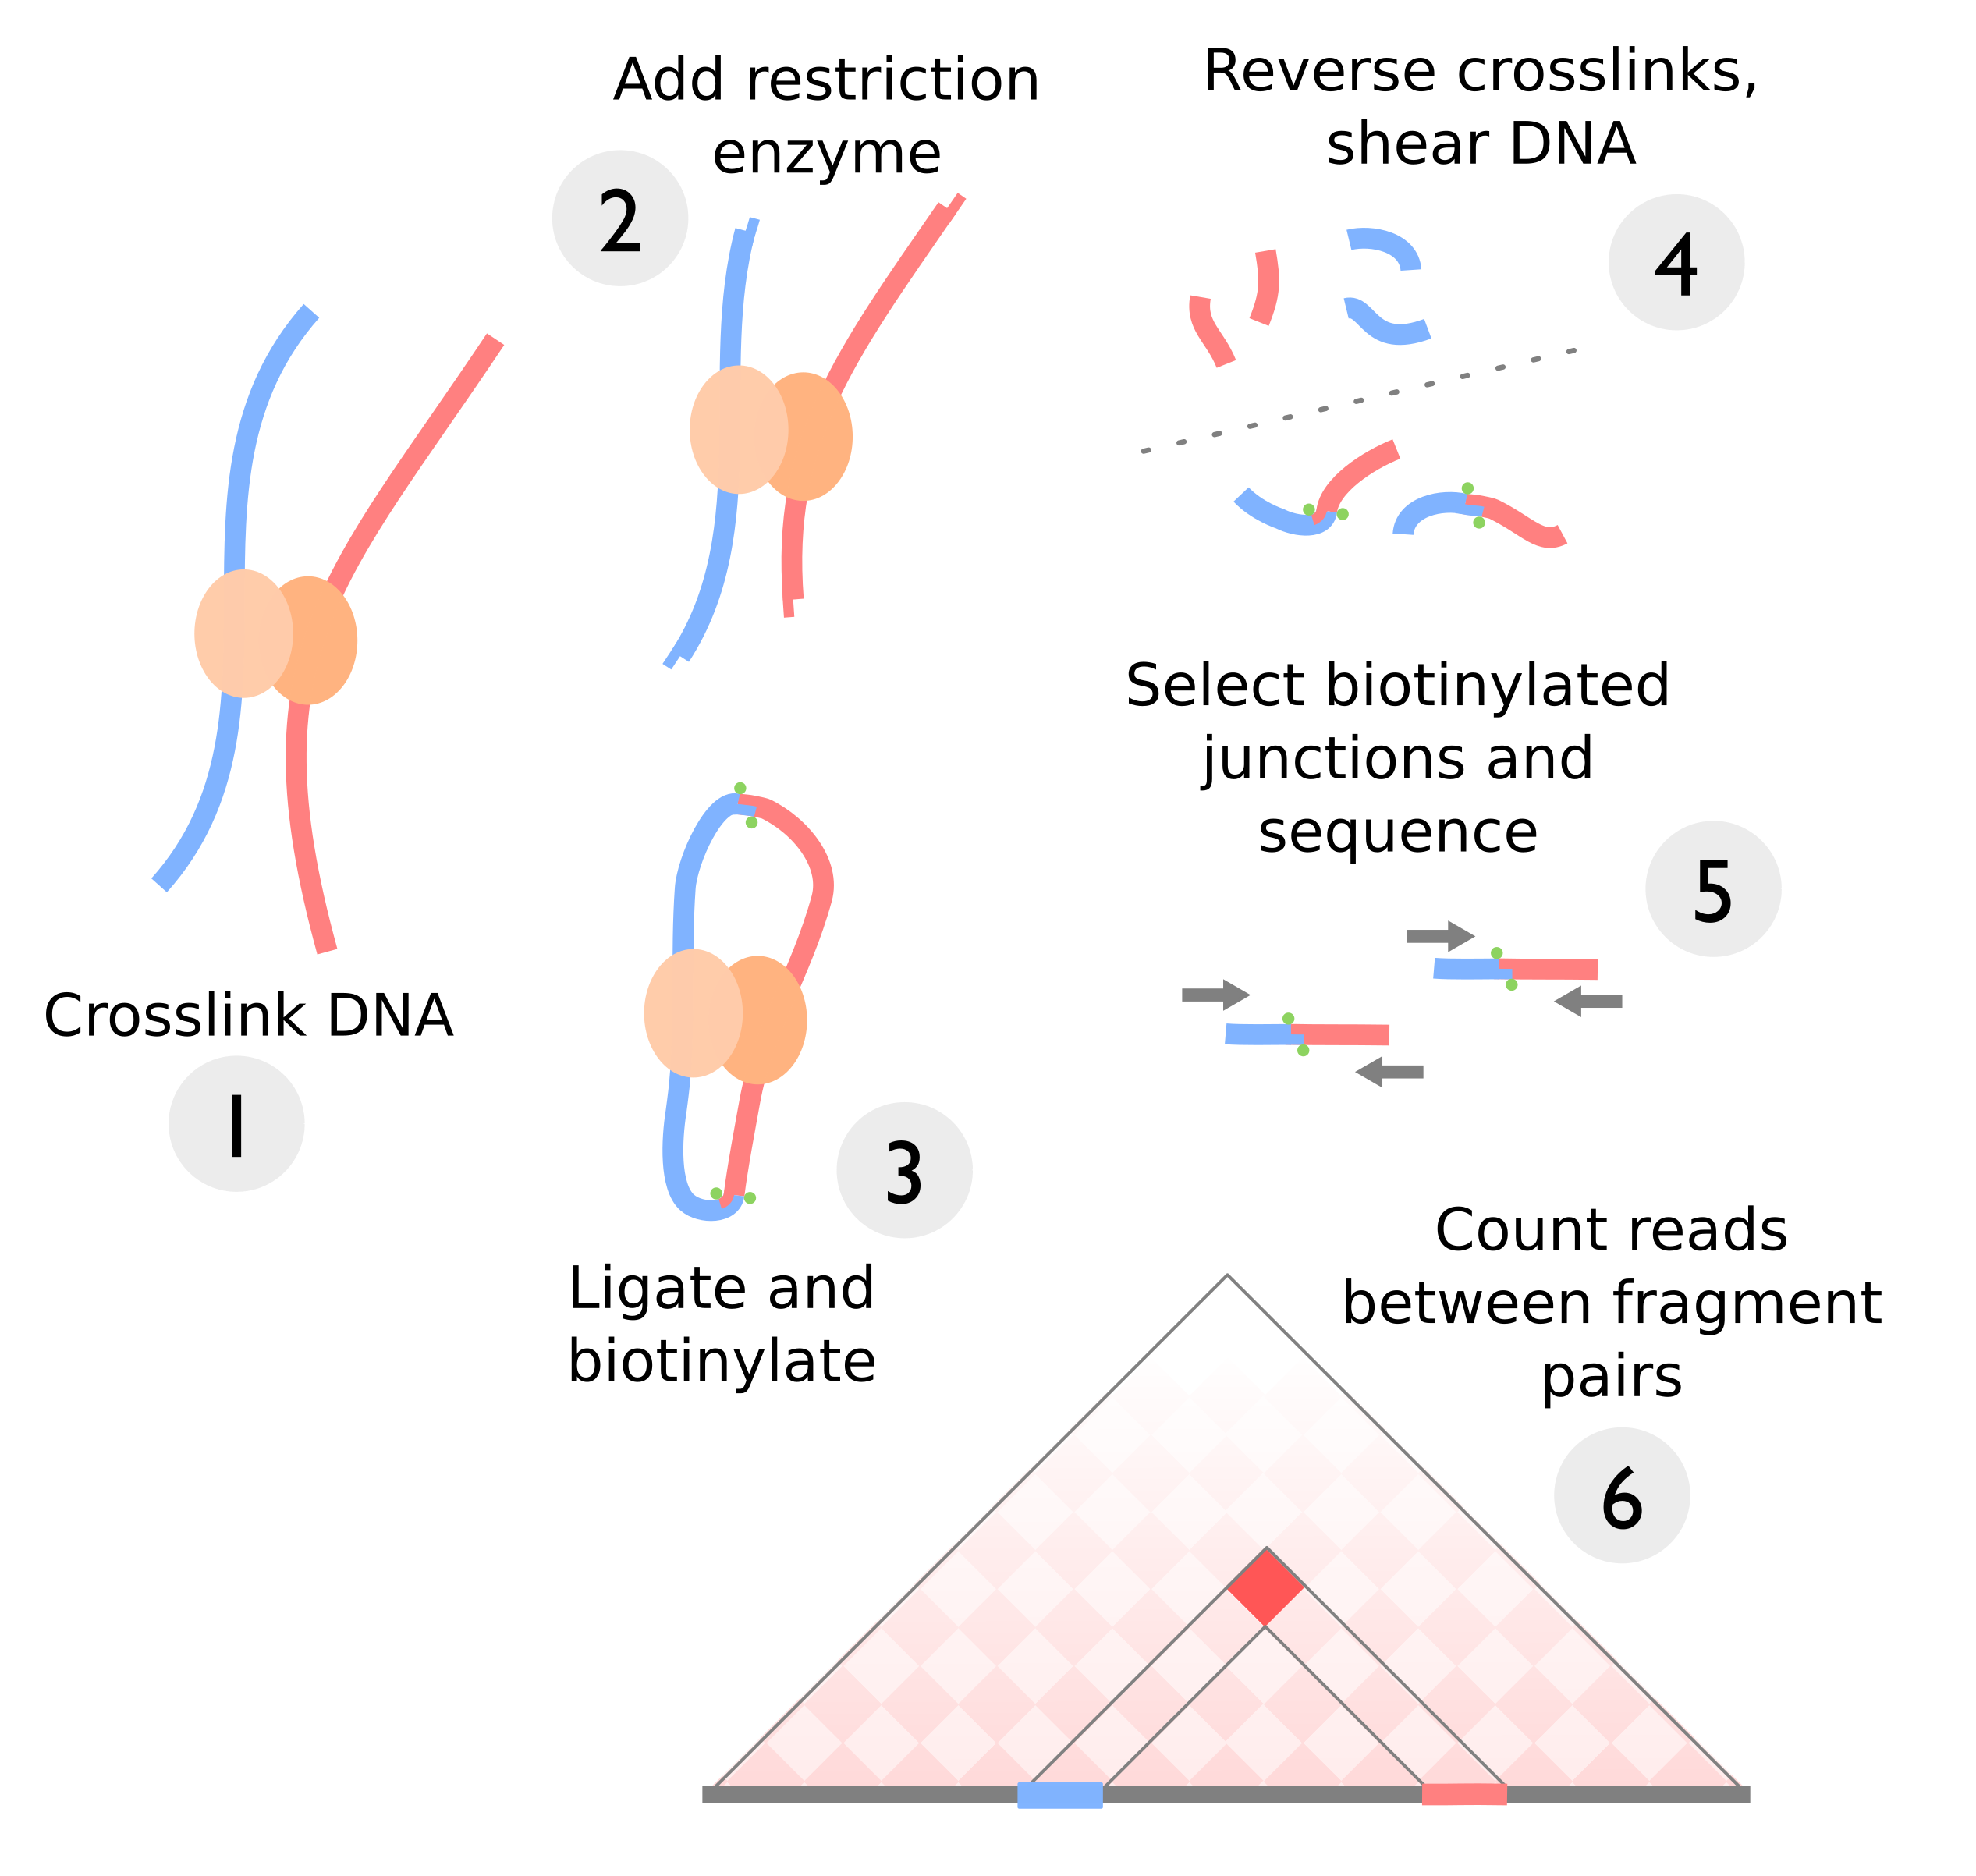
\includegraphics[width=4in]{figs/hic.png}
\captionsetup{width=\textwidth}
\caption[Steps in the Hi-C assay.]{ {\bf Steps in the Hi-C assay. } 
  Schematic of the Hi-C experimental procedure as described in Lieberman Aiden \emph{et al.}\cite{Lieberman2009}
}\label{fig:hicmethod}
\end{center}
\end{figure} 

\subsection{Hi-C variants}\label{sec:hicvar}

The interaction maps produced by Hi-C were found to exhibit several inherent biases. Fragment properties, such as their length, GC content and mappability, were confounding interaction frequency estimates and therefore needed to be normalised-away before subsequent analysis.\cite{Yaffe2011, Hu2013} A range of statistical techniques were developed to correct for these latent variables,\cite{Imakaev2012, Dekker2013, Hu2012, Li2014} while experimentalists instead looked to improve on the experimental procedure itself.

Tethered chromosome capture (TCC)\cite{Kalhor2012} was the first attempt to increase the signal to noise ratio of Hi-C contacts. In this method, ligations take place on a fixed surface, with the aim of preventing spurious ligations between fragments in solution which were not cross-linked. Kalhor \emph{et al.}\cite{Kalhor2012} reported a large decrease in observed interchromosomal contacts in their tethered library, suggesting many of those originally observed were caused by spurious ligation of non-crosslinked fragments.

Hi-C is a population-level assay, as the retrieved interaction counts are from a huge number of different cells. As well as building population-averaged models of genome structure, it is also of interest to probe cell-to-cell variability through single-cell approaches. For instance, it's been estimated that long-range contacts identified with C-methods may occur in as few as $10\%$ of cells at any one time.\cite{VanSteensel2010} 

In the first single-cell Hi-C study, Nagano \emph{et al.}\cite{Nagano2013} aimed to explore this cell-to-cell variability by performing the Hi-C assay on single, hand-selected nuclei. An obvious limitation this Hi-C variant is that a single restriction fragment can ligate to at most one other fragment, meaning even if $100\%$ yield were to be achieved, any $n \times n$ restriction fragment interaction matrix could at most populate $\frac{n}{2}$ cells; in practice, the realised yield of this first single cell Hi-C experiment was just $2.5\%$.\cite{Nagano2013} Nevertheless, single-cell Hi-C was able to reproduce findings from population-based (or ``ensemble") Hi-C, such as preferential interactions between active domains, but also was able to dissect \emph{trans} interactions, suggesting high cell-to-cell variability leads to their relatively uniform appearance in normal Hi-C interaction maps.\cite{Nagano2013} Combined with observations from TCC which gave evidence that interchromosomal contacts were disproportionately the result of spurious ligation,\cite{Kalhor2012} the functional significance of these \emph{trans} interactions seems at best unclear in the general case.

Capture-C is another recent Hi-C derivative which attempts to address resolution problems associated with the genome-wide pairwise assay by enriching for promoter-enhancer interactions using \emph{a priori} selection.\cite{Mifsud2015} It could be said that Capture-C is to Hi-C as exome-capture sequencing is to a whole-genome approach. Indeed, a suggestion in the original Hi-C paper was that resolution could be improved by either increased sequencing or using hybrid capture.\cite{Lieberman2009}

Use of a cell population also averages away cell-cycle effects, with the vast majority of results coming from cells during interphase (around $97\%$\cite{Naumova2013}). Naumova \emph{et al.}\cite{Naumova2013} looked to assay chromosome conformation specifically over different cell cycle stages, to better understand chromosome compaction during mitosis.

In-site Hi-C was a recent refinement of the Hi-C method, from the published of the original method.\cite{Rao2014} The principle difference is that fixation and ligation now happen in place, within intact cell nuclei.

\subsection{Chromosome compartments}\label{sec:compartments}

In the paper describing the Hi-C technique,\cite{Lieberman2009}  Lieberman-Aiden \emph{et
  al.} described low-resolution structures they name  ``A'' and ``B'' nuclear compartments. These are regions with a median size of around 5 megabases which showed properties typical
of euchromatin and heterochromatin, respectively. A compartments were observed through 3D-FISH to be centrally-positioned in the nucleus and  ChIP-seq data showed several hallmarks of transcriptional activity. B compartments, conversely, were heterochromatic and lamina-associated regions, with little transcription and repressive histone modifications such as H3k9me3.\cite{Lieberman2009, DeWit2012} As expected from positioning data, the co-location of compartment types is also visible in their contact maps. 

\begin{figure}
\begin{center}
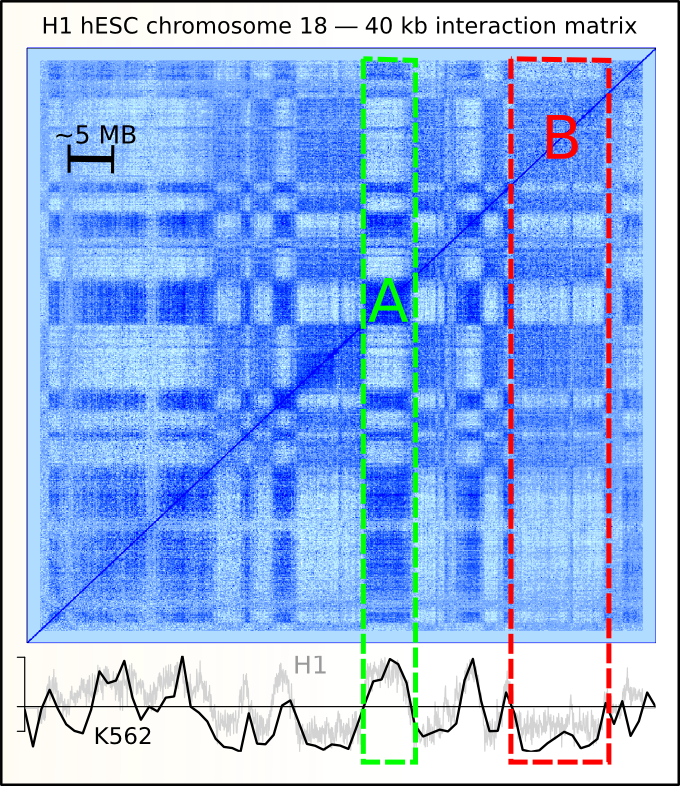
\includegraphics[width=.75\textwidth]{figs/eigcalc.png}
\captionsetup{width=\textwidth}
\caption[Derivation of A/B compartment profile from Hi-C data.]{ {\bf Derivation of A/B compartment profile from Hi-C data.} 
Observed interaction frequencies (O) are averaged along super-diagonals to give a distance-normalised expected matrix (E). The Pearson correlation of the O/E matrix then can undergo eigenvector expansion; in most cases eigenvector $\mathbf{v}$ with the largest eigenvalue, $\lambda$, then reflects A/B compartmentalisation.\cite{Lieberman2009}
}\label{fig:eigcalc}
\end{center}
\end{figure} 

These compartments were identified through a continuous eigenvector profile, derived from a normalised Hi-C contact matrix.\cite{Lieberman2009} Importantly, this measure holds more information than a simple two-state classification, rather the continuous values can be interpreted as relative levels of compaction or activity.\cite{Dekker2013, Imakaev2012}

\subsection{Topological domains}\label{intro:tads}

The falling cost of high-throughput sequencing enabled increasingly deep sequencing of Hi-C experiments. Sequencing is the main resolution-limiting resource for this assay, as to increase the analysis resolution and maintain the level of coverage requires an exponential increase in the total amount of sequencing required.\cite{Lieberman2009, Tanay2013}

In experiments totalling around two billion total sequencing reads, Dixon \emph{et al.}\cite{Dixon2012} produced Hi-C contact maps in human and mouse cell lines at 40 kb resolution. The authors noticed smaller domains they designated "topological associative domains" (or TADs) which were observable as self-interacting, off-diagonal blocks of higher-than-expected self-interaction frequency. They defined a domain calling algorithm based on the directional bias of a genomic region's contacts, and used a Hidden Markov Model to infer blocks of strongly up- or downstream-biased, reasoning that domain boundaries are present when a strongly upstream biased region is adjacent to a region of opposite bias (Fig. \ref{fig:dicalc}). These boundaries themselves were investigated and were found to display suggestive functional enrichments for DNA binding proteins including CTCF, long thought to act as an insulator of chromatin state.

\begin{figure}
\begin{center}
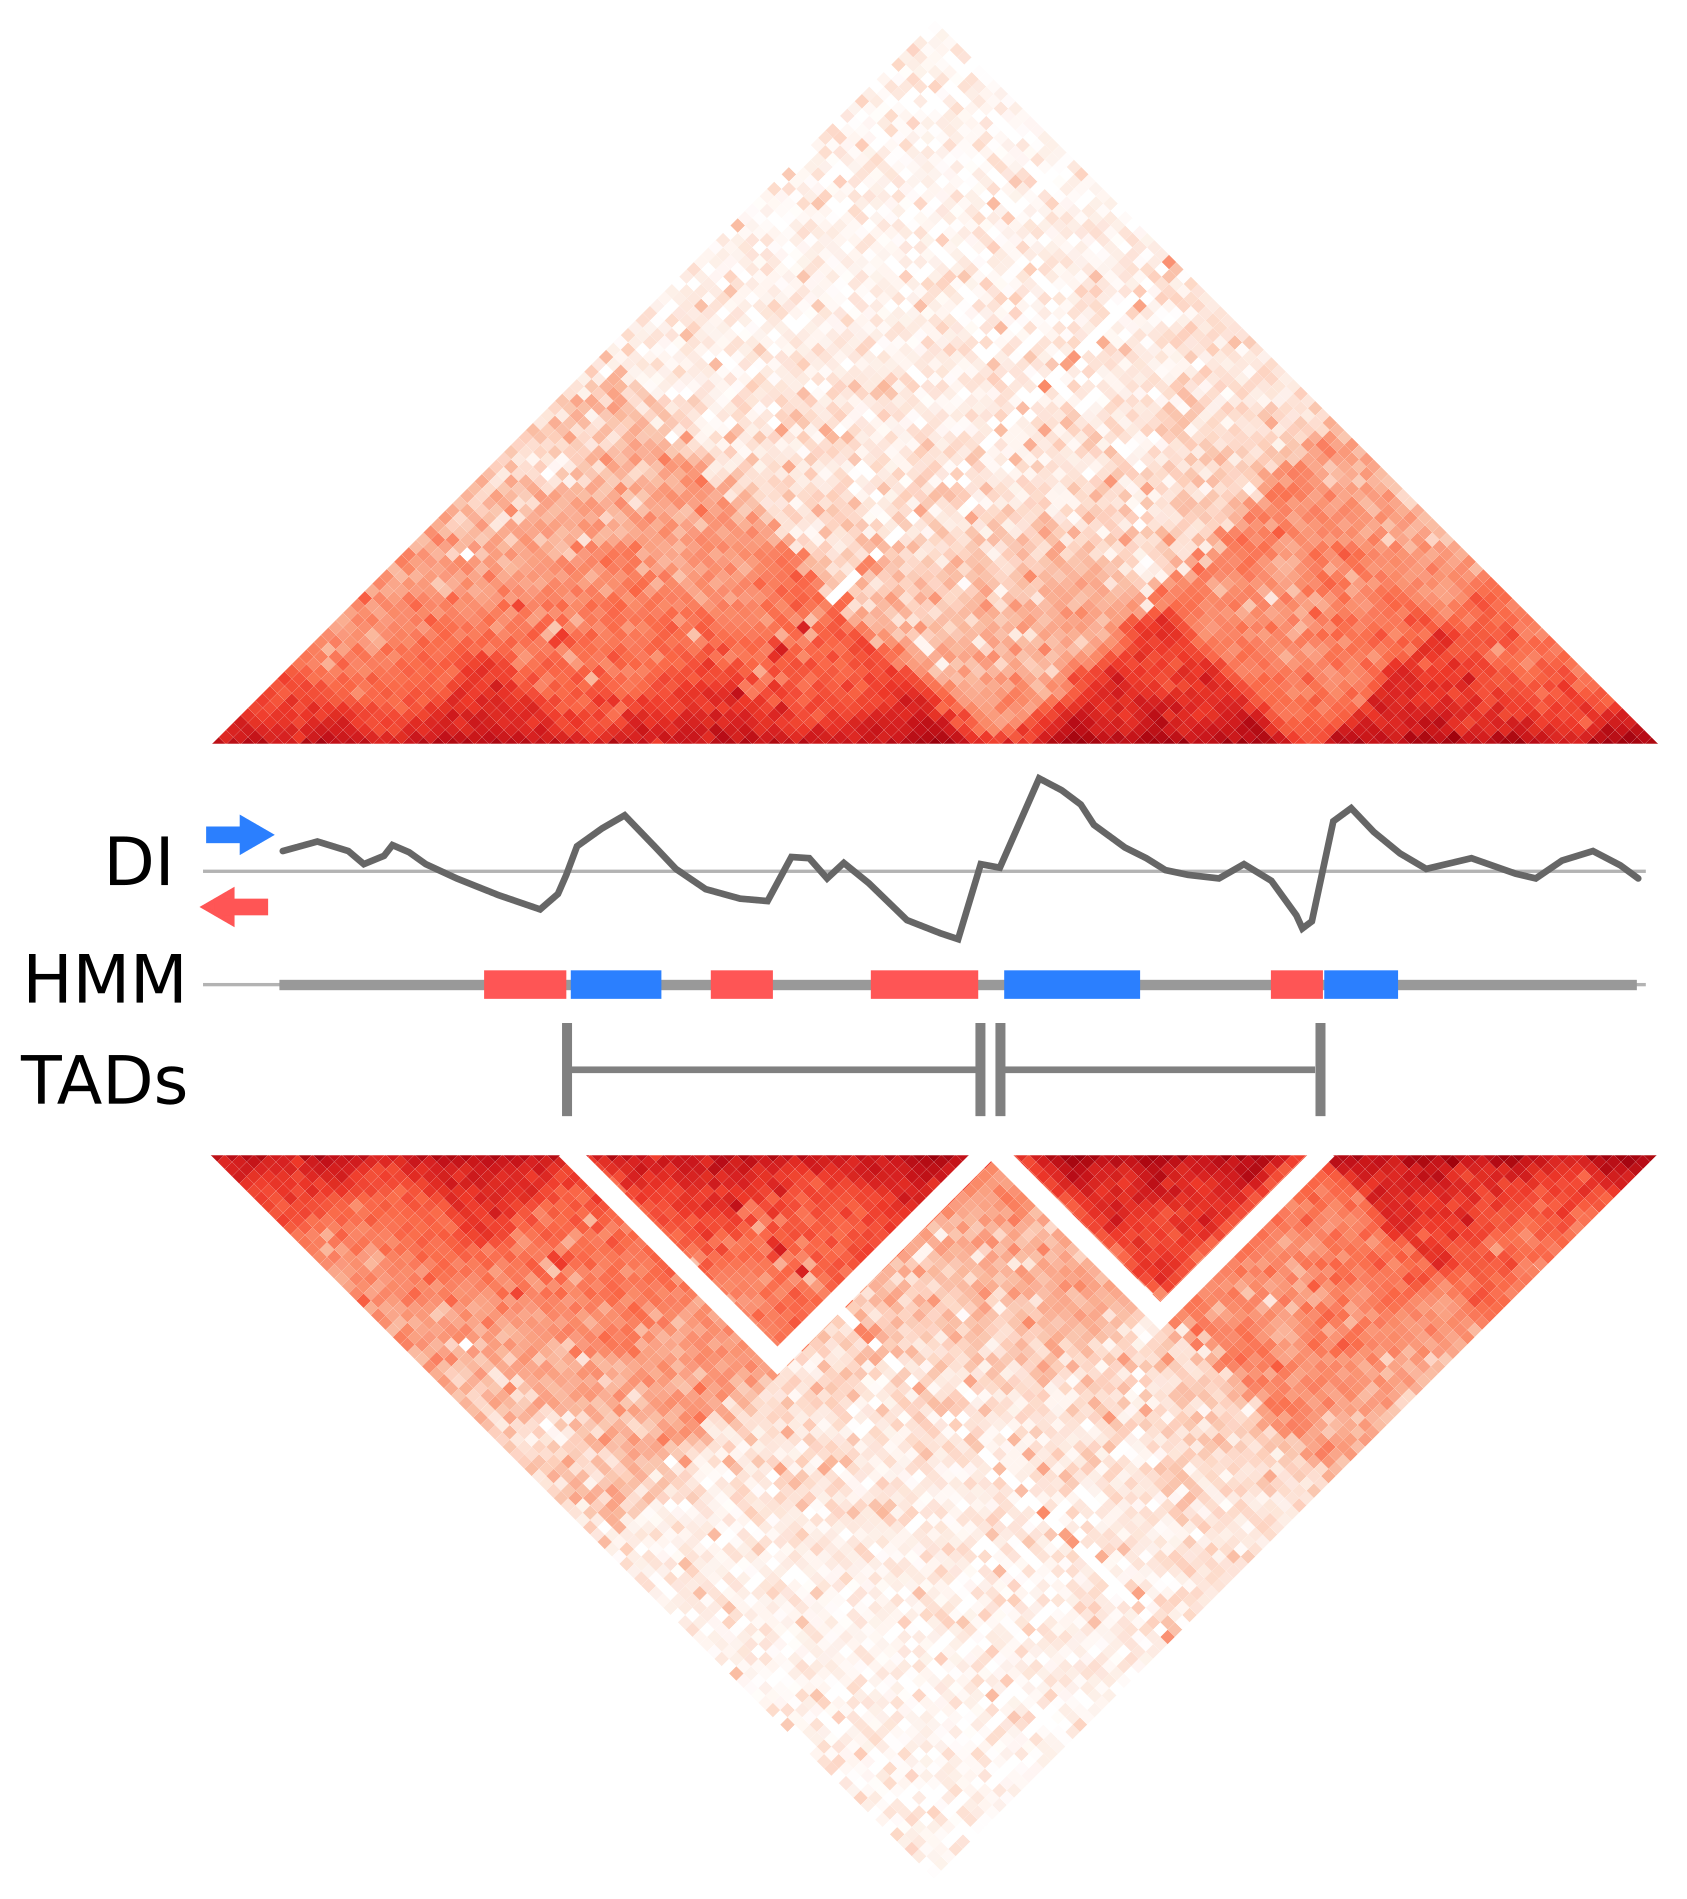
\includegraphics[width=2.5in]{figs/di_example.png}
\captionsetup{width=\textwidth}
\caption[Dixon \emph{et al.} pipeline for calling topological associating domains (TADs).]{ {\bf Dixon \emph{et al.} pipeline for calling topological associating domains (TADs).} First a directionality index (DI) is calculated for each bin based on the ratio of upstream:downstream contacts. Secondly a Hidden Markov Model (HMM) is used to infer the most likely state sequence that emitted the DI variable. Finally a simple rule is applied whereby a run of high-confidence upstream-biased state calls marks the end of a domain. New domains begin with any subsequent downstream-biased state. Gaps between TAD calls can be observed, and as labelled border regions up to a size threshold of 400 kb, whereafter those regions are unclassified.\cite{Dixon2012}
}\label{fig:dicalc}
\end{center}
\end{figure} 

Dixon \emph{et al.}\cite{Dixon2012} also performed some comparative analysis, reporting large and significant overlap of domain boundary positions both within species and between human and mouse cell lines.

\subsection{Other proposed structures}

Filippova \emph{et al.}\cite{Filippova2014} developed a tuneable algorithm which identifies "alternative topological domains".

A study of \emph{Drosophila} embryonic chromosomes found a similarly hierarchical organisation of physical domains, and also was able to relate these to ``epigenomics domains" showing specific sets of enrichment signatures representing active, null, polycomb-associated and telomeric regions.\cite{Sexton2012} 

Recent high-resolution studies have been able to resolve ever-smaller levels of sub-structure. Rao \emph{et al.}\cite{Rao2014} refined the concept of chromosome compartments to "sub-compartments", dividing simple A/B divisions into a total of 5 subtypes. The authors were also able to identify "contact domains" of median size 185 kb, many of which were associated with identifiable individual looping events.\cite{Rao2014} The authors also suggest that previously-observed large TADs may be the result of insufficient sequencing; that is, not all boundaries could be detected using 40 kb binned contact maps thus multiple contact domains were unintentionally combined into large domains.

\section{Models of chromatin folding}

Theoretical mechanistic models of chromatin folding such as the
``strings and binders switch'' model\cite{Barbieri2012} and the ``fractal
globule'' model\cite{Lieberman2009, Mirny2011, Grosberg1988a} have both produced simulated data
that reflects empirical C-method observations and potentially describe the polymer
dynamics of chromatin folding.

\subsection{Fractal globule}
Lieberman Aiden \emph{ et al.}\cite{Lieberman2009} tested a number of theoretical models of genome folding to see which best explained the observed power-law scaling between distance and observed contact frequency ($IF =  1 / dist^{-\alpha}$ where $\alpha \approx 1.08$).  The authors sought to distinguish two previously-described models of genome organisation: the "fractal globule" and "equilibrium globule". The authors found that a theoretical fractal globule, embodying scale-independent self-similar aggregate folding, better fit the observed data than an equilibrium globule null model where simulated polymer folding was allowed to proceed unchecked.

% cartoon of fractal globule ?

The fractal globule model was noted for its appealing functional properties. Under this model, for example, the polymer folds are knot-free hence could facilitate local dynamics of repression and activation without wider disruption. Despite this appeal, the authors were careful to state that while their simulations show good agreement with observed data, this does not preclude other organisational models from having similar or greater explanatory power.\cite{Lieberman2009}

\subsection{Strings and binders switch}

Subsequent modelling techniques integrated known biological phenomena as well as polymer models. This formed the basis of Barbieri \emph{et al.}'s\cite{Barbieri2012} ``strings and binders switch" (SBS) model, where the authors simulated polymer folding in the presence of DNA binding factors, such as the known genome organiser CCCTC-binding factor (CTCF).\cite{Phillips2009} This organisational model was developed in an attempt to consolidate global Hi-C measures of contact scaling with C-based experiments on smaller regions and FISH studies, which found a range of scaling parameters. The authors also explore the different values of $\alpha$ between cell lines and even chromosomes, and find that their mechanistic model can explain each case using variable concentrations of binders which causes phase-switching between open and compacted chromatin, with fractal globule existing at the phase transition boundary.

This model offers broad explanatory power for a range of observed power law coefficients ($\alpha$) and from simple underpinnings, but critics point out that simulations were performed on a polymer composed of just 500 monomers.

\subsection{Looping}

\subsection{Cell cycle changes}

Chromosome structure has been assayed both through mitosis\cite{Naumova2013} and 
Studies have also focused on the edge-case of chromatin structures on X-chromosomes. 

\section{Criticisms of C-methods}

% resolution
The resolution of a Hi-C experiment has a hard-limit imposed by the choice of restriction enzyme. For example, the commonly-used HindIII enzyme is a six-cutter that recognises the motif AAGCTT and cuts approximately every 4 kb, on average.\cite{DeWit2012} More recent studies have switched to a four-cutter restriction enzyme, for example MboI,\cite{Rao2014} which increases this upper-bound on resolution to the order of hundreds of basepairs (i.e. naively, $4^{4} = 256$bp fragments, on average). A downside of using more frequent restriction enzymes is the potential side-effect of promoting more non-specific ligations by increasing the concentration of fragments in solution.\cite{Rao2014} 

% For 
% in Lieberman: s^{1/3}  == scaling observed in 3D FISH (500 kb < 2 Mb)
A key consideration with C-methods is that, when accurately stated, the assays are measuring ``the frequency at which sequences are ligated together by formaldehyde cross-linking",\cite{Williamson2014} which is then assumed to be a proxy for physical distance within the nucleus. This is a marked difference from aforementioned FISH methods, where the physical distance is observed directly, albeit through the addition of non-native probes. So strong is this assumption, that methods have been developed that use a known FISH distance to then calibrate genome-wide Hi-C distances,\cite{Shavit2014} yet it remains unclear to what extent these two methods are compatible.

%Incidental contacts
When interpreting C-methods data it should also be kept in mind that even verifiable contacts are by no-means functional. To elaborate, C-methods may find two regions to be strongly co-localised, but an understanding of the region may explain their co-localisation to be caused by mutual interaction with a nuclear lamina or nucleolus, for example, rather than any specific functional relationship between the two loci.\cite{Dekker2013} In addition, a functional enhancer--promoter interaction will necessarily constrain the contacts of other nearby regions, potentially causing highly-reproducible "bystander interactions"\cite{Dekker2013} that are nevertheless uninteresting form a functional perspective. 

% something about polymer folding, unavoidable contacts between nearby regions? Refs in Dekker2013: http://www.nature.com/nrg/journal/v14/n6/full/nrg3454.html#ref24

An additional and separate issue identified with C-methods, specifically 3C in this instance, emerges from reports that the observed ligation frequency is as low as $1\%$ of expected values in a model system,\cite{Gavrilov2013} potentially magnifying the relative influence of noise and artefacts.

\section{Machine learning in genomics}

Machine learning offers a powerful framework for understanding complex datasets, such as those produced in large-scale genomics studies. Problems in the field such as gene prediction and inferring regulatory networks can be approached by employing a learning algorithm, either in a supervised way based on a known truth set, or through unsupervised methods aimed at pattern detection or clustering (for reviews see \citenum{Jordan2015, Libbrecht2015}). If a successful predictive model can be built, it can then be dissected to explore statistical rules which may impart novel biological insight. As a toy example, learning a highly-accurate model of enhancer prediction could itself identify novel epigenetic marks indicative of enhancers, generating testable hypotheses about how enhancers are activated.

The link between epigenomic features and local chromatin state has been
analysed computationally in a number of publications, notably in
developing the
Hidden Markov Model-based ChromHMM\cite{Ernst2012} algorithm which predicts states such as active promoters and enhancers, using a
range of histone marks and other underlying features.\cite{Ernst2011} Similarly a Random Forest-based
algorithm was developed to predict enhancers from histone
modification data.\cite{Rajagopal2013} However few studies have spanned all of
these levels of chromatin structure and nuclear organisation, and it is not yet known how locus-level chromatin features may
be related to higher order genome organisation. \\

\subsection{ENCODE}

The Encyclopaedia of DNA Elements (ENCODE) is a consortium project started over a decade ago with the ambitious aim of comprehensively cataloguing all functional elements in the human genome.\cite{Feingold2004, Qu2013, Dunham2012} This project involves huge amounts of data production from a diverse array of experimental methods, such as: ChIP-seq, DNase-seq, RNA-seq, CAGE, DNase-seq and ChiA-PET.\cite{Myers2011} Importantly these methods were applied to a range of human cell types, including many well-studied immortalised cell lines as well as primary cells and tissues, and according to standardised experimental methods\cite{Landt2012} coupled with statistical quality control\cite{Dunham2012, Boyle2014, Marinov2013} to ensure data is comparable between different data produces and of consistently-high accuracy. 

Despite ENCODE's human-focus, there also exists spin-off projects aimed at building similar genomics resources for mouse\cite{Yue2014} and, more recently, \emph{Drosophila} and \emph{C. elegans}.\cite{Ho2014} Together these data sources offer an unparalleled resource for comparative and within-species genomics research, and as such have been used in at least 1200 publications to date.\cite{encodenews}

Data generated by ENCODE consortium members has a proven utility in genomics research. 
% First SegWay, chromHMM, then predictive ML
Notable two ENCODE-associated groups have released models which classify the human genome into discrete "chromatin states", such as actively transcribed regions or gene promoters. The first, named \texttt{SegWay}, trained a dynamic Bayesian network on  31 ENCODE-generated input variables and called an unsupervised 25-state genome segmentation in the ENCODE pilot region.\cite{Hoffman2012} Independently another chromatin state predictor named \texttt{ChromHMM} was developed.\cite{Ernst2011, Ernst2012} As the name suggests, this approach instead used multivariate Hidden Markov Models (HHMs) and has the capability to learn a single generative model over multiple cell types. Original runs of the model called 51 chromatin states using over 40 input features,\cite{Ernst2010a} but more recently these two methods were combined to call a consensus set of just 7 chromatin states.\cite{Hoffman2013} This discretisation of the chromatin landscape greatly helps interpretability, at the cost of simplifying the complex underlying data series, and is used for this reason later in this work (Section XX). 

More broadly, ENCODE data has been used by external researchers to generate input variables for machine learning-based predictive models which describe transcriptional output,\cite{Cheng2011} gene regulation,\cite{Althammer2012} and enhancer chromatin states\cite{Rajagopal2013} to name but a few. One such study in particular, that of \citet{Dong2012}, is reproduced and further analysed in this work (Section XX) and is used as a template for our own machine learning framework (Section XX). We also make use of ENCODE data in other chapters (e.g. \ref{chap:boundaries}) due to its comprehensive coverage of model human cell types and stringent data production guidelines referenced above.


The recent comprehensive ChIP-seq datasets
produced by the ENCODE consortium\cite{Dunham2012} combined with Hi-C
genome-wide contact maps in a number of human cell
types\cite{Dixon2012, Lieberman2009, Kalhor2012} present a remarkable
opportunity to investigate the relationships between local
chromatin features and higher order structure.

In this work, a machine-learning approach was employed to model the
compartmental characteristics of large genomic regions based on their
aggregate levels of various histone marks and DNA binding
proteins. Dissection of the resulting models was then used as a
means of gleaning biological insights into the basis of higher order
structure and of highlighting important differences between cell types.

% machine learning schematic for (e.g.) chromHMM ?

\section{Aims}

In the broadest terms, the aims of this work are to investigate the relationship between structure and function of the genome. In particular, we aim to answer the following questions: 
\begin{enumerate}
\item How does higher order chromatin structure compare across cell types?
\item Can we predict higher order chromatin structure from locus-level features?
\item How do the characteristics of boundaries remarking higher order domains vary between cell types and domain classes?
\end{enumerate}


\ifstandalone
\begin{small}
\bibliography{/Users/benmoore/Documents/library,/Users/benmoore/Documents/customrefs}
\end{small}
\fi

\end{document}
